\chapter{New Revolutions in Particle Physics: Standard Model}

We begin where Leonard Susskind begins: not with an abstract statement of the Standard Model, but with the fermion table and with the concrete actions of the gauge groups on that table. These notes follow the lecture closely, as curated by LazyingArt LLC, and keep its main pedagogical thread in view. Weak interactions are indeed weak, but not because the weak coupling is absurdly small. The real suppression comes from the propagator of a very heavy \(W\) boson. Only after that argument has been made does the lecture turn, qualitatively, toward spontaneous symmetry breaking.

\section{Gauge Symmetries on the Fermion Table}

The lecture opens by reconstructing the fermion table as an operational object. Quarks are arranged horizontally by family and vertically by color. The first point is that the symmetry groups are understood through what they do to these slots.

\begin{itemize}
\item \(SU(3)\) acts vertically: it mixes red, green, and blue while leaving the family label unchanged.
\item \(SU(2)\) acts horizontally within a weak doublet: it moves us between \(u\) and \(d\), between \(c\) and \(s\), and between \(t\) and \(b\), while leaving color unchanged.
\item \(U(1)\) acts by phase: every charge-carrying field is multiplied by the appropriate phase factor.
\end{itemize}

Thus the lecture packages the Standard Model, at this stage, as
\begin{equation}
SU(3)\times SU(2)\times U(1).
\end{equation}
The product structure is the important point: the color transformations do not change upness and downness, and the weak transformations do not change color.

Susskind insists on a physical reading of this structure. The generators of a gauge symmetry are not merely algebraic decorations; the gauge bosons are their physical manifestation. A gluon emission does exactly what an infinitesimal color transformation does. If a red up quark emits the appropriate gluon and becomes a green up quark, then the gauge boson has enacted one of the generators of \(SU(3)\). The same gluon acts on every row. One and the same color generator changes a red top quark into a green top quark just as it changes a red up quark into a green up quark.

The same language is then transferred to the weak interaction. A \(W\) boson enacts the horizontal move:
\begin{equation}
u \to d + W^+,
\qquad
d \to u + W^-.
\end{equation}
Gluons never move us horizontally. \(W\) bosons never move us vertically. That directional distinction is one of the lecture's organizing ideas.

\section{From Quarks to Weak Processes}

Once the horizontal action has been identified, the lecture immediately asks how far it extends. It extends beyond quarks. Leptons fit the same family pattern, but they do not carry color, so they do not participate in the \(SU(3)\) interaction. Weakly, however, they sit in analogous doublets.

What matters for \(W\) emission in this lecture is the charge difference across the doublet. For quarks,
\begin{equation}
Q(u)-Q(d)=\frac{2}{3}-\left(-\frac{1}{3}\right)=1.
\end{equation}
For the electron-neutrino pair,
\begin{equation}
Q(\nu_e)-Q(e^-)=0-(-1)=1.
\end{equation}
So the same \(W\) structure that connects \(u\) to \(d\) can connect \(\nu_e\) to \(e^-\). The weak interaction, as presented here, cares about the correct charge difference, not about whether the doublet is made of quarks or leptons.

The lecture then fixes one concrete process and stays with it:
\begin{equation}
d \to u + W^-,
\qquad
W^- \to e^- + \bar{\nu}_e,
\end{equation}
so that at the hadronic level we obtain neutron beta decay,
\begin{equation}
n \to p + e^- + \bar{\nu}_e.
\end{equation}
Inside the neutron, one down quark turns into an up quark, while the spectator quarks merely carry the neutron into a proton.

\begin{figure}[htbp]
\centering

\includegraphics[width=0.88\textwidth]{lecture_06_figure_03.png}
\caption{Weak-interaction board sketches across both panels. The screenshot is best read as evidence for the lecture's board layout and process organization rather than as a perfectly legible standalone derivation.}
\end{figure}

The board image is worth keeping, because it records the lecture's layout. But the clean mathematical content is the process topology itself, which we can redraw without pretending that every board label is fully legible.

\begin{figure}[htbp]
\centering
\begin{tikzpicture}[scale=1.0]
\draw[->] (-3,1) -- (-1.3,1) node[midway,above] {$d$};
\fill (-1.1,1) circle (0.05);
\draw[->] (-1.1,1) -- (0.8,1.9) node[midway,above] {$u$};
\draw[->] (-1.1,1) -- (0.7,0.2) node[midway,below] {$W^-$};
\fill (0.9,0.2) circle (0.05);
\draw[->] (0.9,0.2) -- (3.0,0.9) node[midway,above] {$e^-$};
\draw[->] (0.9,0.2) -- (3.0,-0.4) node[midway,below] {$\bar{\nu}_e$};
\node at (-2.3,1.7) {$n$};
\node at (0.2,2.5) {$p$};
\end{tikzpicture}
\caption{A clean redraw of the weak process underlying neutron beta decay, suppressing spectator-quark bookkeeping.}
\end{figure}

At this point the lecture pauses over coupling strengths. Electromagnetically, the relevant small number is the fine-structure scale,
\begin{equation}
e^2 \sim \alpha.
\end{equation}
Strong emission is much more probable, so the strong coupling is much larger in practice. But the crucial surprise is that the weak coupling is not parametrically tiny in comparison with \(e\). At the rough level of the lecture,
\begin{equation}
g_w^2 \text{ is of the same general order as } e^2.
\end{equation}

\subsection{Question \& Answer}

\paragraph{Question.} If the weak coupling \(g_w\) is not especially small, why are weak interactions weak?

\paragraph{Answer.} Because the vertex is only part of the story. A Feynman diagram contains vertices and propagators. The weak vertex alone does not explain the long neutron lifetime. The missing suppression comes from the propagation of a very heavy intermediate \(W\).

\section{Propagators in Distance Space and Natural Units}

The lecture now changes gears. A Feynman diagram is not only a statement about interaction vertices; it also contains the amplitude for a particle to move from one point to another. That is the propagator. In position space we call it \(\Delta\), and the lecture treats it first as a function of distance.

At short distance the propagator is large. For the massless-style behavior that Susskind sketches, it falls by a power law,
\begin{equation}
\Delta(d)\propto \frac{1}{d^2}
\qquad
\text{for small } d.
\end{equation}
If the exchanged particle had no mass, the power law would simply continue. But for a massive particle the story changes. Beyond a characteristic distance scale, the propagator falls exponentially. The lecture does not derive the exact special-function form; it keeps the point qualitative, and so shall we:
\begin{equation}
\Delta(d) \text{ falls exponentially once } d \text{ reaches the inverse mass scale.}
\end{equation}

To identify that scale, the lecture introduces natural units. The blackboard writes
\begin{equation}
c=\hbar=1,
\qquad
[m]=[E]=[p]=[1/\text{length}].
\end{equation}
This is the bridge from dimensional analysis to the physical range of a massive exchange.

\begin{figure}[htbp]
\centering

\includegraphics[width=0.72\textwidth]{lecture_06_figure_02.png}
\caption{Natural-units dimensional relations and qualitative propagator falloff. The screenshot is retained because the lecture ties the units statement directly to the distance-space sketch.}
\end{figure}

Since length has units of inverse mass, the only distance scale we can build from a mass \(m\) is
\begin{equation}
d \sim \frac{1}{m}.
\end{equation}
Restoring the constants gives the familiar Compton scale,
\begin{equation}
d \sim \frac{\hbar}{mc}.
\end{equation}
That is where the massive propagator begins to dive.

\begin{figure}[htbp]
\centering
\begin{tikzpicture}[scale=1.0]
\draw[->] (0,0) -- (6.6,0) node[right] {$d$};
\draw[->] (0,0) -- (0,4.8) node[above] {$\Delta(d)$};
\draw[thick] plot[smooth] coordinates {(0.35,4.4) (0.8,3.2) (1.4,2.5) (2.2,1.9) (3.2,1.5) (4.4,1.15) (5.8,0.9)};
\draw[thick,red] plot[smooth] coordinates {(0.35,4.4) (0.8,3.2) (1.4,2.5) (2.2,1.9) (3.0,1.55) (3.6,1.05) (4.2,0.45) (4.8,0.18)};
\node at (5.3,1.35) {$m=0$};
\node[red] at (4.6,0.75) {$m\neq 0$};
\draw[dashed] (3.4,0) -- (3.4,1.45);
\node at (3.4,-0.35) {$d\sim 1/m$};
\end{tikzpicture}
\caption{A schematic redraw of the lecture's distance-space picture: power-law behavior at short distance, and sharp exponential suppression once the mass scale is felt.}
\end{figure}

Heavier particles have shorter effective range in this sense. That is already the qualitative answer to why a heavy \(W\) does not mediate weak processes very efficiently over the scales relevant to nuclear physics.

\section{Momentum-Space Propagator and the Low-Energy Weak Estimate}

The lecture then makes the move that experiments force upon us. In the laboratory we do not usually know the spacetime separation between emission and absorption points. We know momenta. So we pass to the Fourier transform of the propagator.

Let \(k\) denote the momentum carried by the exchanged \(W\). The lecture's simplified low-energy convention is
\begin{equation}
\widetilde{\Delta}_W(k)=\frac{1}{k^2+m_W^2}.
\end{equation}
For a photon, which has no mass,
\begin{equation}
\widetilde{\Delta}_\gamma(k)=\frac{1}{k^2}.
\end{equation}

\begin{remark}
The lecture is deliberately using the low-energy, mostly space-like form of the propagator. The point here is not full Minkowski-signature bookkeeping, but the fact that the denominator is dominated by \(m_W^2\) in beta decay.
\end{remark}

Now we have the promised worked estimate. In neutron beta decay there are two weak vertices and one \(W\)-propagator. Therefore
\begin{align}
\mathcal{A}_{n\to p e^- \bar{\nu}_e}
&\sim g_w \,\widetilde{\Delta}_W(k)\, g_w \\
&\sim \frac{g_w^2}{k^2+m_W^2}.
\end{align}
But the momentum transfer in beta decay is tiny compared with the mass of the \(W\). Hence
\begin{equation}
k^2 \ll m_W^2,
\qquad
\widetilde{\Delta}_W(k)\approx \frac{1}{m_W^2},
\end{equation}
and so the amplitude reduces to
\begin{equation}
\mathcal{A}_{n\to p e^- \bar{\nu}_e}\sim \frac{g_w^2}{m_W^2}.
\end{equation}
This is exactly the estimate that appears boxed on the blackboard.

\begin{figure}[htbp]
\centering

\includegraphics[width=0.82\textwidth]{lecture_06_figure_04.png}
\caption{Weak-reaction estimate on the board. The boxed factor is spatially separated from the reaction sketch, just as in the lecture: it is an estimate extracted from the process, not a label inside the diagram.}
\end{figure}

We can now square the amplitude to obtain the scale of the probability or rate:
\begin{equation}
P_{\text{weak}}
\sim
|\mathcal{A}|^2
\sim
\frac{g_w^4}{m_W^4}.
\end{equation}
That is the mathematical spine of the lecture. Weak interactions are weak because the exchanged boson is heavy. The heavy \(W\) suppresses low-energy exchange.

Historically, old weak-interaction experiments did not have enough momentum transfer to see the denominator vary with \(k\). They only saw the low-energy combination
\begin{equation}
G_F \sim \frac{g_w^2}{m_W^2},
\end{equation}
the Fermi constant. Only later, with enough energy and momentum, did one see that the effective weak strength is really momentum-dependent, because the underlying propagator is
\(\bigl(k^2+m_W^2\bigr)^{-1}\).

\section{Virtual Exchange and Energy Conservation}

The lecture now turns interpretive again, and quite rightly so. The formula is not yet the whole understanding. One must still answer the natural question: if the \(W\) is so heavy, how can it appear at all in beta decay?

\subsection{Question \& Answer}

\paragraph{Question.} How can a heavy \(W\) appear when the neutron does not have enough energy to emit a real on-shell \(W\)?

\paragraph{Answer.} It cannot appear as a real external particle. It appears only as a virtual intermediate state, and then only for a very short time. The lecture encodes that limitation by the energy-time uncertainty estimate
\begin{equation}
\Delta E\,\Delta t \lesssim \hbar.
\end{equation}
If an intermediate state carries an excess energy \(\Delta E\), it must disappear again within a time of order
\begin{equation}
\Delta t \lesssim \frac{\hbar}{\Delta E}.
\end{equation}
So the heavy \(W\) is not produced as a long-lived free particle in neutron decay. It is a short-lived internal fluctuation.

The lecture explains this with the tunneling analogy. Consider a particle initially at rest in a potential well. The far side of the barrier is chosen so that the potential energy there is the same as at the starting point. Classically the particle cannot cross the barrier. Quantum mechanically it can tunnel. In the barrier region, if we insist on describing the process in classical language, the particle seems to carry too much potential energy. That apparent violation is tolerated only briefly.

\begin{figure}[htbp]
\centering

\includegraphics[width=0.72\textwidth]{lecture_06_figure_06.png}
\caption{Potential barrier and equal-energy tunneling points. The lecture uses this picture to make the short-lived virtual intermediate state intelligible without turning the analogy into ontology.}
\end{figure}

\begin{figure}[htbp]
\centering
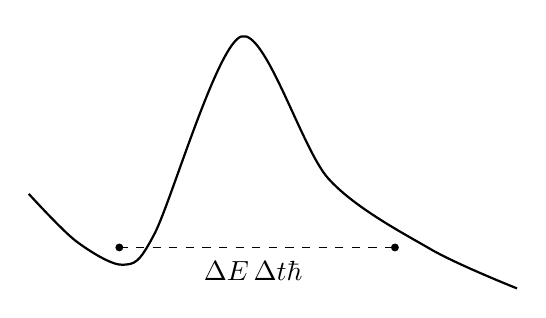
\begin{tikzpicture}[scale=1.0]
\draw[thick] plot[smooth] coordinates {(0.4,1.4) (1.0,0.8) (1.6,0.5) (2.0,0.9) (3.1,3.4) (4.2,1.6) (5.5,0.7) (6.6,0.2)};
\draw[dashed] (1.55,0.72) -- (5.05,0.72);
\fill (1.55,0.72) circle (0.05);
\fill (5.05,0.72) circle (0.05);
\node at (3.25,0.42) {$\Delta E\,\Delta t \lesssim \hbar$};
\end{tikzpicture}
\caption{A schematic redraw of the tunneling analogy: the two marked points have the same total energy, while the barrier region represents the classically forbidden intermediate stage.}
\end{figure}

The same logic is then transferred back to the weak interaction. There is not enough energy in neutron decay to emit a real \(W\) and let it fly off. But there is enough for a brief virtual excursion. The intermediate \(W\) must then either be reabsorbed or convert quickly into lighter particles, such as \(e^-+\bar{\nu}_e\).

This point leads to the lecture's clean distinction between real and virtual particles.

\begin{definition}
In the language of Feynman diagrams, the real particles are the incoming and outgoing asymptotic states. Virtual particles are the internal lines that appear inside the amplitude and are not themselves observed as final free particles.
\end{definition}

Energy conservation remains exact from the full initial state to the full final state. The apparent violation belongs only to the intermediate off-shell description. If one supplies enough external energy to resolve that short time scale, one no longer has the same process. One has created a different process in which a real \(W\) can appear in the final state, decay with its own short proper lifetime, and exhibit ordinary time dilation when boosted.

Susskind also emphasizes a general lesson here. The rate of a process is controlled by three things:
\begin{itemize}
\item coupling constants,
\item masses, or equivalently the propagators built from them,
\item available energy.
\end{itemize}
The suppression of weak decay comes primarily from the second item, while the possibility of the process at all still depends on the third.

\section{The Missing Third Weak Boson}

Only after all of this does the lecture return to a loose end in the group theory. If the weak interaction is really based on \(SU(2)\), then the gauge bosons must match the generators. But
\begin{equation}
\dim SU(2)=3.
\end{equation}
Two charged bosons,
\begin{equation}
W^+,\qquad W^-,
\end{equation}
cannot be the whole story. There must be a third weak gauge boson. The lecture stops short of working it out and points forward instead: the missing neutral boson is related to the \(Z\), and the precise relation between electric charge, the weak group, and the neutral boson is postponed to the next lecture.

This brief return is important. It reminds us that the product-group slogan \(SU(3)\times SU(2)\times U(1)\) is already slightly more subtle than the first table-based picture suggested.

\section{Spontaneous Symmetry Breaking}

The lecture then changes subject, but in a deliberately unfinished way. We are given not a derivation of the Higgs mechanism, but a qualitative doorway into spontaneous symmetry breaking.

The first illustration is the dinner-table story: a perfectly symmetric arrangement, but an unstable choice between left and right. Once the instability is tipped, the whole system settles one way. The more serious example is a lattice of two-state variables, which Susskind is happy to describe either as spins or as classical coins. Neighboring variables prefer to align. Thus the local energy satisfies, schematically,
\begin{equation}
E_{\text{parallel}} < E_{\text{anti-parallel}}.
\end{equation}
But the two fully aligned states are degenerate:
\begin{equation}
E(\text{all heads}) = E(\text{all tails}).
\end{equation}
So the system has two ground states, not one.

That is the essential structure. The microscopic rules are symmetric under heads \(\leftrightarrow\) tails, but the state in which the system settles need not display that symmetry. A tiny bias imposed far away can select one of the two vacua. After that selection has occurred, local excitations are measured relative to the chosen vacuum.

\subsection{Question \& Answer}

\paragraph{Question.} How is spontaneous symmetry breaking different from explicit symmetry breaking?

\paragraph{Answer.} In explicit symmetry breaking the local rules are already biased. If a single head carried lower energy than a single tail, then the symmetry would be broken in the Hamiltonian itself, and there would be only one preferred vacuum. In spontaneous symmetry breaking the local rules remain symmetric, the vacua remain degenerate, and it is the choice of ground state that breaks the symmetry.

This distinction has a physical consequence, and the lecture insists on it. In the spontaneous case, if one imposes heads far away on one side of space and tails far away on the other, the minimum-energy configuration contains a boundary between the two regions. That boundary is a domain wall. Domain walls are therefore the qualitative signal that one is dealing with spontaneous, not explicit, breaking.

The lecture stops here on purpose. It does not yet derive the Higgs mechanism. It only places the reader in the right conceptual terrain: a symmetric theory, a degenerate set of ground states, an instability that chooses one of them, and a coming return to the electroweak problem through that lens.

\section{Summary}

The lecture begins with the fermion table and turns the slogan \(SU(3)\times SU(2)\times U(1)\) into concrete moves on that table. It then shifts from symmetry to dynamics by asking why weak interactions are weak. The answer is not a tiny bare weak coupling. The answer is the propagator of a very massive \(W\), which at low momentum yields the suppression
\[
\mathcal{A}_{\text{weak}} \sim \frac{g_w^2}{m_W^2},
\qquad
P_{\text{weak}} \sim \frac{g_w^4}{m_W^4}.
\]
From there the lecture clarifies what a virtual particle is, why exact energy conservation is never abandoned, and why a tunneling picture is a useful but limited analogy. It closes by pointing to two unfinished revolutions: the missing neutral weak boson, and spontaneous symmetry breaking, whose full electroweak significance is reserved for the next lecture.